%CLASSE DOCUMENTO - LINGUA E DIMENSIONE FONT
\documentclass[12pt]{toptesi}

%%%%%%%%%%%%%%%%%%%%%%%%%%%%%%%%%%%%%%%%%%%%%%%%%%%%%%%%%%%%%%%

% INCLUSIONE PACCHETTI
\usepackage[utf8]{inputenc} %utf8
\usepackage[italian]{babel}
\usepackage[T1]{fontenc}
\usepackage{blindtext}
\usepackage{graphicx,wrapfig}
\usepackage{booktabs}
\usepackage{lmodern}
\usepackage{varioref}
\usepackage{url}
\usepackage{array}
\usepackage{paralist}{\obeyspaces\global\let =\space}
\usepackage{verbatim} 
\usepackage{subfig}
\usepackage{tabularx}
\usepackage{amsmath}
\usepackage{amsfonts}
\usepackage{float}
\usepackage{amssymb}
\usepackage{multicol}
\usepackage{multirow}
\usepackage{listings}
\usepackage[pass]{geometry}
\usepackage[figuresright]{rotating}
\usepackage{algorithm}
\usepackage{algorithmic}
\usepackage{amsmath}
\usepackage[babel]{csquotes}
\usepackage{hyperref}
\usepackage[backend=bibtex]{biblatex}
\usepackage{pdfpages} 
\usepackage{pythonhighlight}
%%%%%%%%%%%%%%%%%%%%%%%%%%%%%%%%%%%%%%%%%%%%%%%%%%%%%%%%%%%%%%%

% CONFIGURAZIONE LINK E RIFERIMENTI
\hypersetup{%
    pdfpagemode={UseOutlines},
    bookmarksopen,
    pdfstartview={FitH},
    colorlinks,
    linkcolor={black}, %COLORE DEI RIFERIMENTI AL TESTO
    citecolor={blue}, %COLORE DEI RIFERIMENTI ALLE CITAZIONI
    urlcolor={blue} %COLORI DEGLI URL
}

%%%%%%%%%%%%%%%%%%%%%%%%%%%%%%%%%%%%%%%%%%%%%%%%%%%%%%%%%%%%%%%

% CONFIGURAZIONE LISTATI/CODICE - CANCELLARE SE NON NECESSARIO
% PYTHON - BIANCO E NERO
\lstset{%
	captionpos=b,
	language=Python,
	basicstyle =\small\ttfamily,
	keywordstyle=\color{black}\bfseries,
	breaklines=true,
	breakatwhitespace=true,
	frame=lines,
	numbers=left,
	numberstyle=\footnotesize,
}

%%%%%%%%%%%%%%%%%%%%%%%%%%%%%%%%%%%%%%%%%%%%%%%%%%%%%%%%%%%%%%%

% FRENCHSPACING VA _SEMPRE_ ABILITATO PER DOCUMENTI IN ITALIANO
\frenchspacing

%%%%%%%%%%%%%%%%%%%%%%%%%%%%%%%%%%%%%%%%%%%%%%%%%%%%%%%%%%%%%%%

%DEFINIZIONE SEZIONI IN NUMERAZIONE ROMANA
%ELENCO DEI LISTATI/CODICI
\makeatletter
\newcommand\listofcodes{%
 \iffrontmatter\else\frontmattertrue\fi
 \if@openright\cleardoublepage\else\clearpage\fi
 % change the meaning of \chapter in a group
 \begingroup\def\chapter##1{\@schapter}
 \phantomsection % for the hyperlink
 \lstlistoflistings 
 \endgroup
} 
\makeatother

%%%%%%%%%%%%%%%%%%%%%%%%%%%%%%%%%%%%%%%%%%%%%%%%%%%%%%%%%%%%%%%

% INFORMAZIONI PDF - PERSONALIZZARE
\pdfinfo{%
  /Title    (Senza carta igienica)
  /Author   (Tinaso de Tinasis)
  /Subject  (Un trattato di toccante urgenza)
  /Keywords (LaTeXi carta igienica urgenza Politecnico Presicce)
}

% %%%%%%%%%%%%%%%%%%%%%%%%%%%%%%%%%%%%%%%%%%%%%%%%%%%%%%%%%%%%%%%

% % FRONTESPIZIO - PERSONALIZZARE
% % ELIMINATE LE VOCI CHE NON VI SERVONO

% % UNIVERSITA - NOME
% \ateneo{Università degli Studi di Bergamo}

% % FACOLTA - DICITURA - CANCELLARE O DECOMMENTARE
% %\FacoltaDi{Faculty of}
% % FACOLTA - NOME
% \facolta{Ingegneria}

% % CORSO DI LAUREA - DICITURA (MANTENERE LO SPAZIO) - CANCELLARE O DECOMMENTARE
% %\CorsoDiLaureaIn{Master of Science in }
% % CORSO DI LAUREA - NOME
% \corsodilaurea{Ingegneria Informatica}

% % TIPOLOGIA TESI
% \TesiDiLaurea{Tesi di Laurea Triennale}

% % TITOLO
% \titolo{Senza carta igienica}

% % SOTTOTITOLO
% \sottotitolo{Un trattato di toccante urgenza}

% % RELATORE/I - DICITURA - CANCELLARE SE UN SOLO RELATORE
% %\AdvisorName{Relatori}
% % RELATORE - PROF. NOME E COGNOME
% \relatore{prof.\ Darth Vader}
% % RELATORE AGGIUNTIVO - PROF NOME E COGNOME
% % SE SI HA SOLO UN RELATORE ELIMINARE INSIEME AD AdvisorName
% \secondorelatore{prof.\ Neo Cortex}

% % TUTORE AZIENDALE - TITOLO NOME E COGNOME
% \tutoreaziendale{Ing. Carlino Cane}
% % TUTORE AZIENDALE - DICITURA//AZIENDA
% \NomeTutoreAziendale{Tutore Aziendale\\FeelGood Inc}

% % CANDIDATO - DICITURA (MANTENERE I DUE PUNTI) - CANCELLARE O DECOMMENTARE
% %\CandidateName{Candidate:}

% % CANDIDATO - NOME E COGNOME
% \candidato{Andrea Cattaneo}
% % CANDIDATA - ELIMINARE O SOSTITUIRE CON IL PRECEDENTE
% %\candidata{Tinasa de Tinasis} 
% % SECONDO CANDIDATO - ELIMINARE O DECOMMENTARE
% %secondocandidato{Bombo de Bombis}
% %secondacandidata{Bomba de Bombis}

% % LOGO UNIVERSITA
% \logosede{images/logo}

% % DATA - MESE ANNO
% \sedutadilaurea{Dicembre 2018}

% %%%%%%%%%%%%%%%%%%%%%%%%%%%%%%%%%%%%%%%%%%%%%%%%%%%%%%%%%%%%%%%

% LISTA DEI CAPITOLI DA INCLUDERE - PERSONALIZZARE
\includeonly{%
chapters/chap_intro,%
chapters/chap_tle,%
chapters/chap_protocollo,%
chapters/chap_poc,%
chapters/chap_dimensionamento,%
chapters/chap_analisi_attacchi,%
chapters/chap_possibili_usi,%
}

% FILE DI BIBLIOGRAFIA
\bibliography{bibliography} 


%%%%%%%%%%%%%%%%%%%%%%%%%%%%%%%%%%%%%%%%%%%%%%%%%%%%%%%%%%%%%%%

% INIZIO DOCUMENTO
\begin{document}

% \frontespizio

\includepdf[fitpaper=true,]{frontespizio/fronteingegnerialt.pdf}

%%%%%%%%%%%%%%%%%%%%%%%%%%%%%%%%%%%%%%%%%%%%%%%%%%%%%%%%%%%%%%%

%INTERLINEA - DEFAULT 1 - NON ESAGERATE, NON SUPERATE MAI 1.3 ;)
\interlinea{1.5}

%%%%%%%%%%%%%%%%%%%%%%%%%%%%%%%%%%%%%%%%%%%%%%%%%%%%%%%%%%%%%%%

\frontmatter

% DEDICA - PERSONALIZZARE
% VSPACE - PROPORZIONE USATA PER CENTRATURA VERTICALE DEL TESTO
% FLUSHRIGHT - ALLINEAMENTO ORIZZONTALE A DESTRA
% \vspace*{\stretch{1}}
% \begin{flushright}
% 	\noindent
% 	All'amato me stesso
% \end{flushright}
% \vspace*{\stretch{6}}
% \cleardoublepage


% CITAZIONE - PERSONALIZZARE
% VSPACE - PROPORZIONE USATA PER CENTRATURA VERTICALE DEL TESTO
% FLUSHRIGHT - ALLINEAMENTO ORIZZONTALE A DESTRA
\vspace*{\stretch{1}}
\begin{flushright}
	\noindent
	If I have 300 ideas in a year and
	\\just one turns out to work I am satisfied.

	\textit{Alfred Nobel}
\end{flushright}
\vspace*{\stretch{6}}
\cleardoublepage

%%%%%%%%%%%%%%%%%%%%%%%%%%%%%%%%%%%%%%%%%%%%%%%%%%%%%%%%%%%%%%%

% RINGRAZIAMENTI - PERSONALIZZARE
\ringraziamenti
Grazie a Grazia, Graziella e la sorella.

%%%%%%%%%%%%%%%%%%%%%%%%%%%%%%%%%%%%%%%%%%%%%%%%%%%%%%%%%%%%%%%

% ABSTRACT - PERSONALIZZARE
\sommario
Piacere, sommario.

%%%%%%%%%%%%%%%%%%%%%%%%%%%%%%%%%%%%%%%%%%%%%%%%%%%%%%%%%%%%%%%

% INDICI - ELIMINARE GLI INDICI NON NECESSARI

% INDICE GENERALE
\tableofcontents

% INDICE DELLE FIGURE
\listoffigures

% INDICE DELLE TABELLE
\listoftables

% INDICE DEI CODICI
\listofcodes

%%%%%%%%%%%%%%%%%%%%%%%%%%%%%%%%%%%%%%%%%%%%%%%%%%%%%%%%%%%%%%%

\mainmatter

% INCLUSIONE FILE CAPITOLI - PERSONALIZZARE - TENERE COERENTE CON LISTA IN ALTO
\chapter{Introduzione}
\label{chap:Introduzione}


La Blockchain è uno degli argomenti più caldi nell'industria dell'IT. In questo 
capitolo cercheremo di fare chiarezza, partendo dalle origini di questa tecnologia
sino ad arrivare allo stato dell'arte odierno.

\section{DLT}
Per capire cosa è una \textbf{Distribuited Ledger Technology} è necessario 
innanzitutto chiarire il concetto di Ledger.

Un \textit{Ledger}, parola che in italiano traduciamo come \textit{Libro Mastro}, 
è il registro principale in cui sono riunite tutte le transazioni economiche 
che compongono un dato sistema contabile. Si tratta in sostanza di un documento
nel quale vengono registrate tutte le transazioni economiche, dove viene
indicata la data della transazione, la cifra scambiata e i soggetti coinvolti 
nella transazione (chi dà e chi riceve).

\chapter{Time-Lock Encryption}

\section{Cosa è la TLE}
La \textbf{Time-Lock Encryption} (TLE) (o \textbf{Timed-Release Encryption})
è un metodo per cifrare un messaggio in modo che possa
essere decifrato solo dopo che una certa deadline è stata raggiunta.
Un avversario, anche se ha a disposizione una grande quantità di potenza di calcolo,
non deve essere in grado di ottenere il messaggio prima della deadline.
Inoltre, dopo la deadline i destinatari devono poter leggere il messaggio,
indipendentemente dalla potenza di calcolo che ha a disposizione e
senza dover interagire con il mittente,
con altri riceventi o con terze parti fidate.

Questo tipo di crittografia è molto difficile da ottenere con un modelli
di computazione standard (come la macchina di Turing), perché questi non mettono
a disposizione un "orologio del mondo reale" affidabile.
Nel capitolo \ref{chap:protocollo} proponiamo una soluzione che si appoggia sui DLT,
i quali mettono a disposizione
le buone proprietà di cui necessita la Time-Lock Encryption.

Il problema dell'\textit{invio di un messaggio nel futuro} è stato proposto per la prima volta
da May \cite{May:time-released-crypto} nel 1993 e
successivamente studiato da Rivest, Shamir and Wagner \cite{Rivest96time-lockpuzzles}.

La Time-Lock Encryption ha diverse applicazioni nel mondo reale. Queste verranno
discusse nel dettaglio nel capitolo \ref{chap:possibili-usi}.

\section{Requisiti}
Ricapitolando, un buon sistema di TLE deve soddisfare i seguenti requisiti.

\subsection{Certezza di pubblicazione del messaggio al tempo $ \tau $}
Un buon sistema di TLE deve garantire che il messaggio venga pubblicato al

\subsection{Segretezza del messaggio sino al tempo $ \tau $}
\label{subsec:segretezza-tle}


\section{Come implementare la TLE}
Sostanzialmente esistono due strategie
per affrontare questo problema

\subsection{Time-Locked Puzzle}
I Time-Locked puzzle sono stati introdotti per la prima volta
da Merkle \cite{Merkle:1978:SCO:359460.359473} e approfonditi
da Bellare et. al. \cite{Bellare:1996:EKE:888619}
e da Rivest et. al. \cite{Rivest96time-lockpuzzles}.
L'idea che sta alla base è quella di trasformare il messaggio ad un certo istante di tempo $ t_0 $
in modo tale che ogni macchina
(seriale o parallela) debba lavorare per un certo quantitativo di tempo $ \Delta $ per risolvere
il problema computazionale sottostante (puzzle). La somma tra $ t_0 $ e $ \Delta $ è la deadline.

Sebbene rappresenti un approccio elegante nell'ambito della teoria della complessità computazionale,
l'uso di \textit{Time-Locked Puzzle} è difficilmente sostenibile nella pratica,
poiché è poco flessibile e richiede l'uso di
grandi quantità di risorse di calcolo. Inoltre è necessario conoscere con
precisione la potenza di calcolo a disposizione del risolutore per poter
dimensionare la difficoltà del puzzle. Generalmente è possibile ottenere
una buona stima di questo valore se ci si basa sull'hardware contemporaneo. È impossibile
invece trovare una stima \textit{future-proof}, poiché non sappiamo quali nuovi strumenti di
calcolo verranno creati nel futuro (es. computer quantistici).
Ad ogni modo, anche se si avesse una stima affidabile a dispozione,
sarebbe possibile garantire solo un limite inferiore
sull'istante di pubblicazione del messaggio, dato che la macchina risolutrice potrebbe per vari motivi
non iniziare immediatamente a lavorare all'istante $ t_0 $,
potrebbe effettuare delle pause durante l'elaborazione
o peggio ancora potrebbe non completare la risoluzione del problema.


\subsection{Trusted agents (agenti fidati)}
\label{subsec:trusted-agents}
Questo approccio si basa su uno o più \textit{agenti fidati} che rilasciano
delle informazioni una volta che si è raggiunta la deadline. Questo può avvenire in
maniera interattiva o non interattiva. Alcuni riferimenti
\cite{time-capsule-signature}, \cite{10.1007/11602897_25}, \cite{10.1007/3-540-48910-X_6},
\cite{10.1007/11889663_17}, \cite{10.1007/978-3-642-15317-4_1}, \cite{10.1145/1330332.1330336}.

I vantaggi di questa strategia sono che non è richiesto che venga effettuata una computazione non-stop,
è possibile di rispettare con precisione la deadline e non è richiesta una stima precisa
della capacità di calcolo dei soggetti coinvolti. Tutto ciò ha un prezzo: gli agenti devono
essere affidabili e devono essere attivi allo scoccare della deadline.


\chapter{Il Protocollo}
\label{chap:protocollo}

In questo capitolo verrà trattato il protocollo proposto per l'implementazione
della Timed-Release Encryption sui DLT.
Cercheremo di spiegare
l'idea che sta alla base con l'ausilio di un esempio.

Rientra nella categoria degli approcci
con \textit{trusted agents} (si veda \ref{subsec:trusted-agents}).
L'idea è quella di distribuire agli agenti gli \textit{share} del messaggio
e sfruttare alcuni smart contract per
fornire loro degli incentivi economici affinché pubblichino lo share
loro assegnato una volta raggiunta la deadline.
La blockchain viene utilizzata come orologio di riferimento
per capire se la deadline è stata raggiunta.

\section{Versione base}
\label{sec:versione-base}
Immaginiamo che Carol abbia bisogno di Timed-Release Encryption su un certo messaggio $ x $.
Per farlo decide farsi aiutare da Alice. Quest'ultima
impegna a conservare il messaggio e a renderlo pubblico solo dopo un
certo istante di tempo $ \tau $.
Diremo che Carol è il \textit{client} e che Alice è l'\textit{agent}.

Alice vuole essere retribuita per la conservazione di $ x $. Viene quindi fissata
una ricompensa \textit{prize}. Chiaramente Alice vuole essere sicura di
ottenere la ricompensa se rispetta il suo impegno. Allo stesso tempo Carol
vuole avere la certezza che Alice possa riscattare il premio solo se si comporta
in maniera corretta.
Carol inoltre non vuole che soggetti terzi partecipino all'accordo, perché desidera
che sia $ x $ sia l'accordo stesso rimangano segreti.
Per ottenere ciò decidono di usare uno smart contract.

\paragraph{Inizializzazione}
Nella fase iniziale Carol comunica il messaggio $ x $ ad Alice. Allo stesso tempo invia
allo smart contract una certa cifra in criptomoneta
che corrispone alla somma tra il \textit{prize} da corrispondere ad Alice e un
\textit{pawn} che le verrà restituito al termine delle operazioni, un hash
crittografico del messaggio $ x $, l'istante di tempo $ \tau $ e una tolleranza $ \delta $.

\begin{figure}[H]
	\centering
	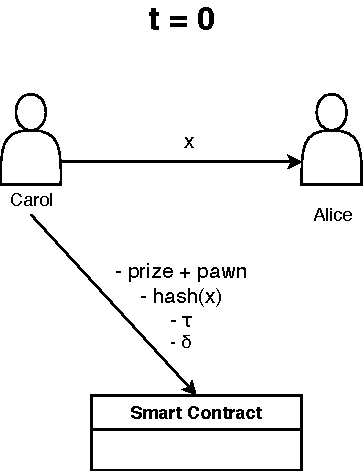
\includegraphics[width=0.3\linewidth]{images/chap_protocollo/base-creazione.pdf}
	\caption{Inizializzazione (versione base)}
\end{figure}

\paragraph{Pubblicazione}
Alice conserva quindi $ x $ e lo rende noto al tempo $ t^{*} $
(con $ \tau \leq t^{*} \leq \tau + \delta $)\footnote{Il $ \delta $ serve a far si che
	Alice pubblichi puntualmente il messaggio. Se non ci fosse questo vincolo temporale
	potrebbe rilasciare il messaggio anche con molto ritardo rispetto a
	$ \tau $ ed ottenere comunque
	la ricompensa.}.
Per farlo invia allo smart contract il messaggio $ x $,
ed in cambio ottiene il suo \textit{prize}.
Allo stesso tempo, Alice riottiene il \textit{pawn}
che aveva versato in precedenza\footnote{
	Il \textit{pawn} è necessario per evitare alcuni comportamenti sleali da parte del client.
	La questione verrà approfondita nella sottosezione \ref{subsec:pawn}}.
\begin{figure}[H]
	\centering
	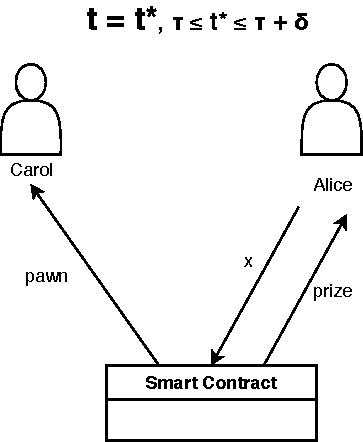
\includegraphics[width=0.3\linewidth]{images/chap_protocollo/base-pubblicazione.pdf}
	\caption{Pubblicazione del messaggio (versione base)}
\end{figure}

\paragraph{Lettura del messaggio}
Dopo il tempo $ t^{*} $, ossia dopo che Alice ha inviato $ x $ allo smart contract,
il messaggio diventa pubblico e
chiunque può leggerlo.
\begin{figure}[H]
	\centering
	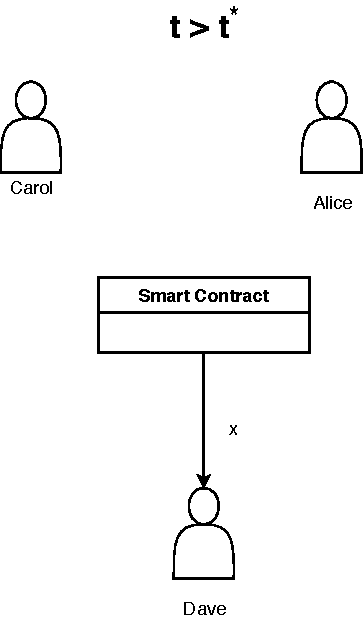
\includegraphics[width=0.27\linewidth]{images/chap_protocollo/base-leggi.pdf}
	\caption{Lettura del messaggio (versione base)}
\end{figure}

\paragraph{Pubblicazione anticipata}
Cosa succede se Alice prova a riscattare il premio prima dell'istante $ \tau $?
Semplicemente lo smart contract rifiuta la sua richiesta.
\begin{figure}[H]
	\centering
	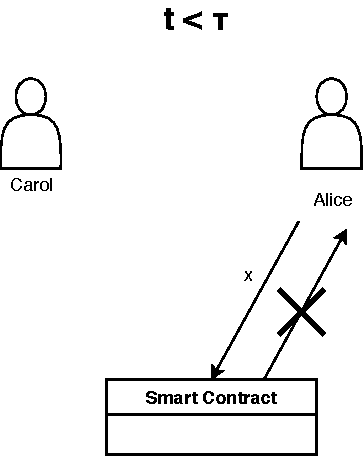
\includegraphics[width=0.3\linewidth]{images/chap_protocollo/base-anticipo.pdf}
	\caption{Tentativo di pubblicazione anticipata (versione base)}
\end{figure}

\paragraph{Leak}
E se Alice cede (volontariamente o a causa di un furto)
il segreto ad Eve prima del tempo $ \tau $?
In questo caso Eve può usare $ x $ per ottenere una ricompensa
\textit{counterprize} \footnote{dove \textit{counterprize} $ \ll $ \textit{prize}.
	Le ragioni di questo vincolo sono spiegate al capitolo \ref{chap:analisi-robustezza}.}
Il riscatto del \textit{counterprize} impedisce ad Alice di ottenere il suo premio.
È evidente che l'interesse di Alice è quello di mantenere $ x $ segreto.
\begin{figure}[H]
	\begin{minipage}{0.4\textwidth}
		\centering
		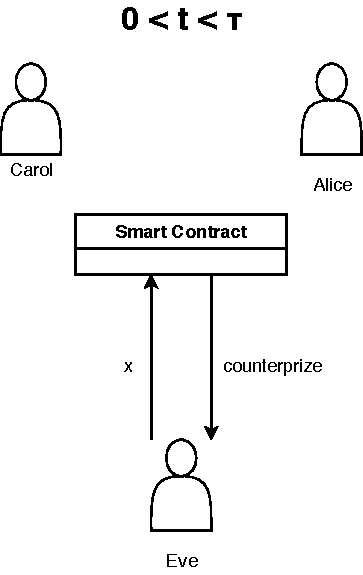
\includegraphics[width=.7\linewidth]{images/chap_protocollo/base-leak-1.pdf}
		\caption{Riscatto del counterprize (versione base)}
	\end{minipage}\hfill
	\begin{minipage}{0.4\textwidth}
		\centering
		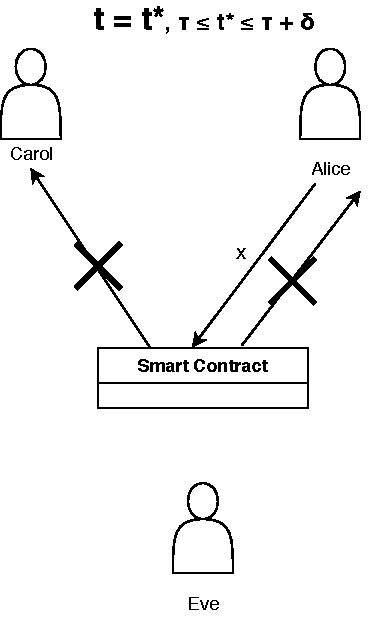
\includegraphics[width=.7\linewidth]{images/chap_protocollo/base-leak-2.pdf}
		\caption{Impossibilità di riscatto del prize (versione base)}
	\end{minipage}
\end{figure}

\section{Versione avanzata}
Facciamo notare che nella versione base
Alice conosce sin
dall'inizio il messaggio
$ x $, perché le è stato affidato nella prima fase del processo.
Ma se Carol volesse che il messaggio rimanga segreto anche ad Alice?
Per soddisfare questa condizione Alice ha bisogno di (almeno) un altro agente,
Bob, e di un
algoritmo di \textit{secret sharing}\footnote{Un algoritmo di secret sharing
	è un algoritmo che permette di
	distribuire un certo segreto tra un gruppo di $ n $ partecipanti, ad ognuno dei quali viene
	assegnato uno \textit{share}. Il segreto può essere ricostruito solo unendo un numero di share
	pari ad un fissato threshold $ t $.}.

\paragraph{Inizializzazione}
Alice, utilizzando un algoritmo di secret sharing, ottiene due share
$ x_A $ e $ x_B $. Invia questi share rispettivamente ad Alice e a Bob ed inizializza
lo smart contract versando due \textit{prize} e due \textit{pawn},
inviando gli hash crittografici
degli share, il tempo $ \tau $ e la tolleranza $ \delta $.
\begin{figure}[H]
	\centering
	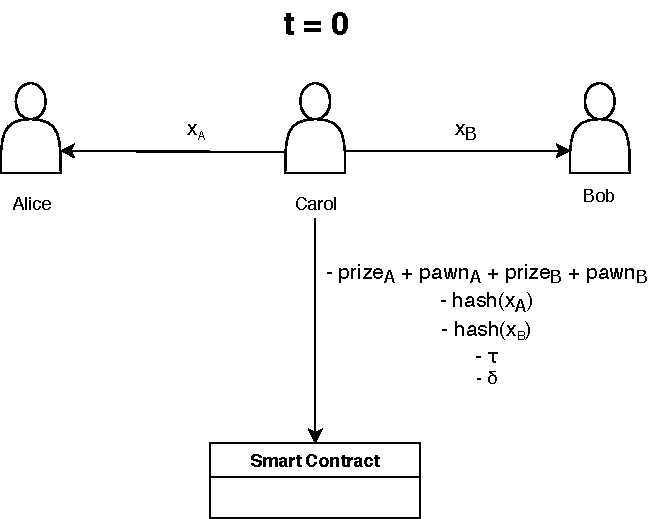
\includegraphics[width=0.6\linewidth]{images/chap_protocollo/avanzato-creazione.pdf}
	\caption{Inizializzazione (Versione avanzata)}
\end{figure}



\paragraph{Pubblicazione}
Alice e Bob pubblicano i loro share rispettivamente al tempo $ t^*_A $ e $ t^*_B $
(con $ \tau \leq t^*_A \leq \tau + \delta $, $ \tau \leq t^*_B \leq \tau + \delta $).
In cambio ottengono i loro
\textit{prize}.
Allo stesso tempo Alice riottiene i rispettivi \textit{pawn} che aveva versato
in precedenza.
\begin{figure}[H]
	\begin{minipage}{0.45\textwidth}
		\centering
		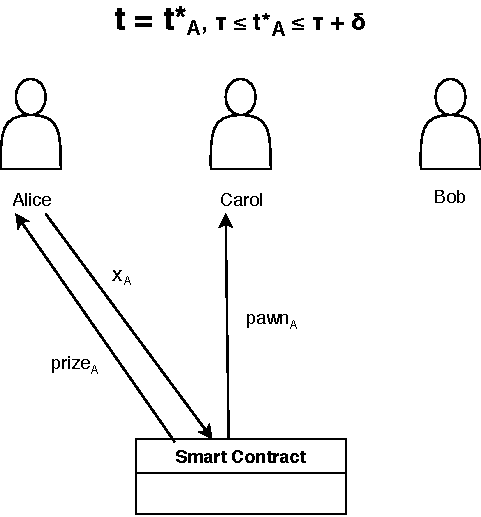
\includegraphics[width=.7\linewidth]{images/chap_protocollo/avanzato-pubblicazione-a.pdf}
		\caption{Pubblicazione dello share $ x_A $ (versione avanzata)}
	\end{minipage}\hfill
	\begin{minipage}{0.45\textwidth}
		\centering
		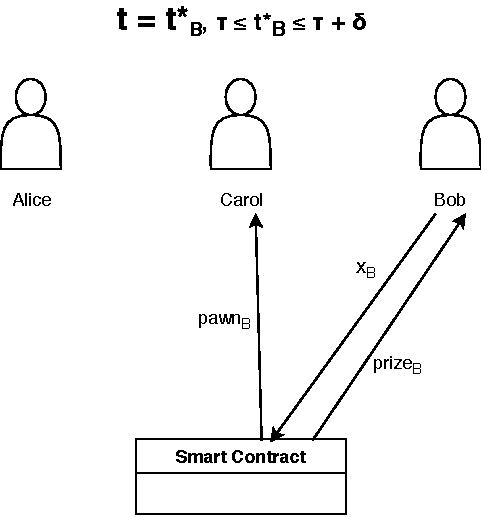
\includegraphics[width=.7\linewidth]{images/chap_protocollo/avanzato-pubblicazione-b.pdf}
		\caption{Pubblicazione dello share $ x_B $ (versione avanzata)}
	\end{minipage}
\end{figure}

\paragraph{Accesso al messaggio}
Dopo il tempo $ t^* = max(t^*_A, t^*_B) $, ossia dopo che sia Alice sia Bob
hanno inviato $ x_A $ ed $ x_B $
allo smart contract, chiunque può leggere gli share dallo smart contract e quindi
ricostruire il messaggio $ x $.
\begin{figure}[H]
	\centering
	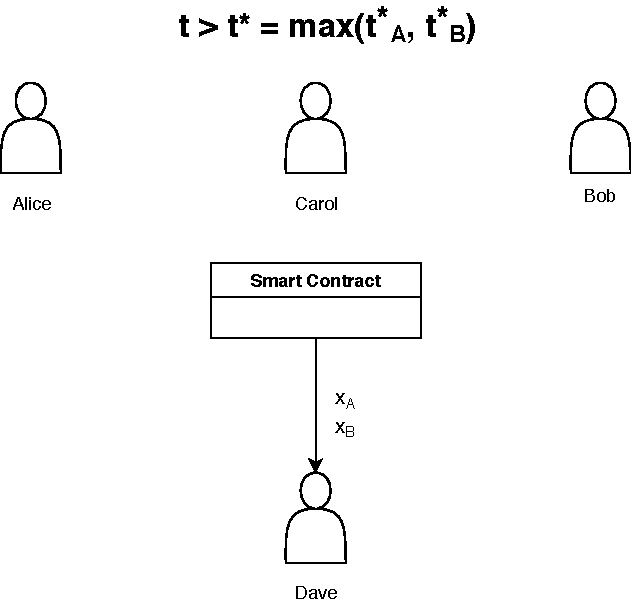
\includegraphics[width=0.5\linewidth]{images/chap_protocollo/avanzato-leggi.pdf}
	\caption{Lettura del messaggio (versione avanzata)}
\end{figure}

\paragraph{Leak}
Cosa succede se Bob cede il suo share ad Eve prima del tempo $ \tau $?
Anche in questo caso Eve può usare $ x_B $ per ottenere una ricompensa
\textit{counterprize}.
Il riscatto del \textit{counterprize} impedisce a Bob di ottenere il suo premio.
Da notare che se Alice si comporta in maniera corretta, ossia se tiene segreto il
suo share, è in grado di ottenere la sua ricompensa indipendentemente dal comportamento
di Bob.
\begin{figure}[H]
	\centering
	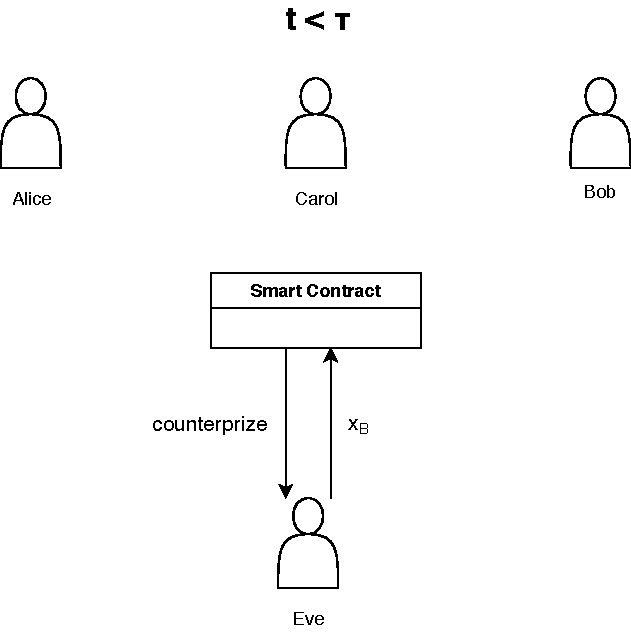
\includegraphics[width=0.4\linewidth]{images/chap_protocollo/avanzato-leak-1.pdf}
	\caption{Riscatto del counterprize (versione avanzata)}
\end{figure}

\begin{figure}[H]
	\begin{minipage}{0.45\textwidth}
		\centering
		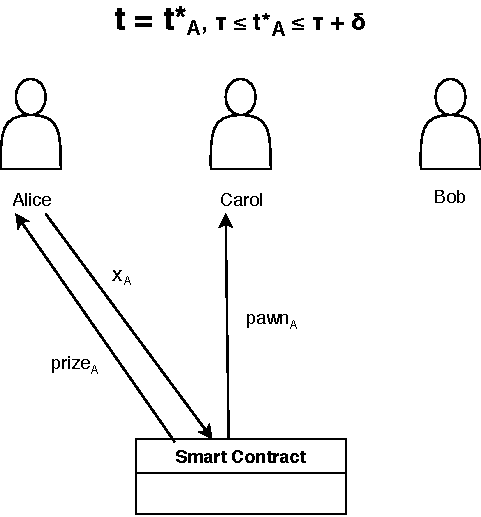
\includegraphics[width=.8\linewidth]{images/chap_protocollo/avanzato-leak-2-a.pdf}
		\caption{Riscatto di $ \text{prize}_A $ (versione avanzata)}
	\end{minipage}\hfill
	\begin{minipage}{0.45\textwidth}
		\centering
		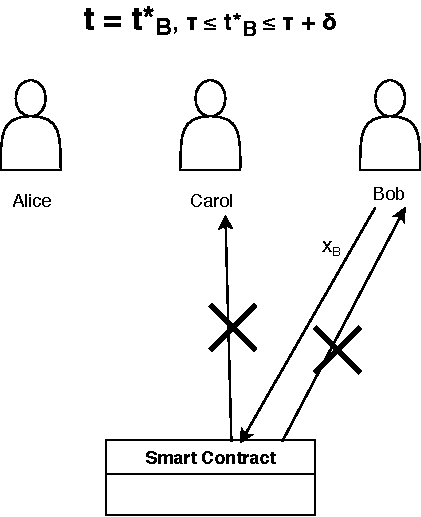
\includegraphics[width=.71\linewidth]{images/chap_protocollo/avanzato-leak-2-b.pdf}
		\caption{Impossibilità di riscatto di $ \text{prize}_B $ (versione avanzata)}
	\end{minipage}
\end{figure}

Abbiamo visto un esempio con la partecipazione di due agenti,
ma il protocollo
può essere analogamente implementato con un numero qualsiasi $ N $ di agenti.


\section{Varianti}
\subsection{Invio del messaggio solo a determinati attori}
Dopo il tempo $ t^* $ il messaggio diventa pubblico a chiunque abbia accesso
allo smart contract. In alcuni contesti questo potrebbe essere un problema, perché
potremmo volere che il messaggio possa essere letto solo da determinati attori.

Una possibile soluzione è aggiungere un layer di cifratura simmetrica al messaggio
prima di criptarlo con la TRE.
La procedura è la seguente.
Per prima cosa si cripta il messaggio $ m $ con cifratura simmetrica e chiave $ k $
ottenendo $ m^\prime $. Allo stesso tempo per ogni account destinatario designato
$ A_1, ..., A_n $ si generano $ k_1, ..., k_n $, dove ogni $ k_i $ è $ k $ cifrato con la
chiave pubblica del portafoglio $ A_i $. A questo punto si genera un header
$ h = (k_1, ..., k_n) $. Infine si crea $ x = (h, m^\prime) $ e lo si utilizza come
segreto per il protocollo proposto.
Una volta raggiunta la deadline $ x $ diventa pubblico, ma $ m $ no. I destinatari designati
$ A_i $ possono leggere $ m $ estraendo $ k_i $ dall'header di $ x $, ottenere
$ k $ decriptandolo con la propria chiave privata e quindi decriptare $ m^\prime $.

\subsection{Divisione di share in più livelli}
La versione avanzata del protocollo proposto può essere estesa con una divisione su più livelli
degli share distribuiti agli agenti.
L'idea è quella di creare un \textit{albero di distribuzione degli share}.
Partendo dal messaggio $ x $, che rappresenta il nodo radice, si ottengono gli share $ x_{1i} $,
rappresentati come nodi figli.
A questo punto su ogni share $ x_{1i} $ si opera nuovamente il protocollo proposto,
utilizzando questa volta $ x_{1i} $ come segreto.
Si ottengono così gli share di secondo livello $ x_{2i} $.
Si può procedere iterativamente in questo modo fino a raggiungere la profondità desiderata.
Gli share nei nodi foglia vengono poi assegnati agli agenti.
Non è strettamente necessario creare un albero bilanciato.

\begin{figure}[H]
	\centering
	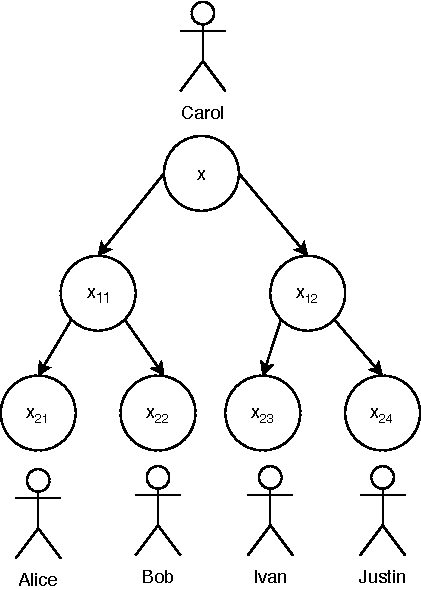
\includegraphics[width=0.45\linewidth]{images/chap_protocollo/protocollo-gerarchia.pdf}
	\caption{Un albero di distribuzione degli share}
\end{figure}

Le scelte progettuali riguardo la struttura dell'albero di distribuzione degli share hanno un
impatto sulla robustezza dell'implementazione del protocollo proposto. Per una analisi più
approfondita rimandiamo al capitolo \ref{chap:analisi-robustezza}.

\subsection{Ricompense intermedie}
Immaginiamo che Carol abbia bisogno di Timed-Release Encryption su un certo messaggio $ x $, e
che la deadline $ \tau $ sia molto avanti nel tempo.
Immaginiamo inoltre che, fissata una ricompensa \textit{prize},
l'agente Alice dia la sua disponibilità, ma a patto di non dover attendere fino al tempo $ \tau $
per riceve l'intera
ricompensa. Una soluzione è quella di prevedere delle ricompense intermedie.
Per realizzarle si procede nel modo seguente.

Il messaggio $ x $ viene diviso in $ n $ share con threshold $ t = n $.
Per ogni share si applica la versione base del protocollo
con deadline $ \tau_1, \tau_2, ... , \tau_n = \tau $
tali che $ \tau_1 < \tau_2 < ... < \tau_n = \tau $ e con rispettive ricompense
$ \textit{prize}_1, \textit{prize}_2, ..., \textit{prize}_n $ tali che
$ \textit{prize}_1 + \textit{prize}_2 +, ... + \textit{prize}_n = \textit{prize} $.
In questo modo l'agente Alice può eseguire delle pubblicazioni intermedie e ricevere le relative
ricompense; allo stesso tempo il messaggio rimarrebbe segreto fino a quando non viene pubblicato
l'ultimo share, ossia fino alla deadline $ \tau $.
Questa metodologia può essere applicata analogamente anche alla versione avanzata.
\chapter{Proof of Concept}

In questo capitolo costruiremo una soluzione sullo Stellar Network
compatibile con il protocollo proposto al capitolo \ref{chap:protocollo}.
Seguirà una Proof of Concept di quanto descritto.

Avremmo potuto proporre una
implementazione anche su altri DLT, come ad esempio Ethereum. Abbiamo scelto
Stellar perché ci da modo di dimostrare che per un'implementazione funzionante
del protocollo proposto non è necessario un ambiente che
offre degli smart contract ``potenti'' come ad esempio
la \textit{Ethereum Virtual Machine},
ma è sufficiente un supporto
``debole'' agli smart contract (si veda \ref{subsec:stellar smart contracts}).


\section{Un'implementazione sullo Stellar Network}
Sia $ U_0 $ il \textit{client};
siano $ U_1, ...\, , U_N $ gli \textit{agenti} e
siano rispettivamente $ S_1, ...\, , S_N $ i segreti assegnati agli agenti
(share o messaggi).

Per prima cosa $ U_0 $ crea gli account $ A_1, ...\, , A_N $ e
versa su questi account una cifra pari alla somma tra
il \textit{prize}, il \textit{pawn} e il costo che dovrà sostenere per le commissioni
delle transazioni che dovrà effettuare.
% TODO
% Per il calcolo delle commissioni si rimanda
% alla sezione \ref{sec:calcolo-commissioni}

A questo punto per ogni account $ A_i $ il client crea $ N $ transazioni
ognuna delle quali rivolta ad uno degli utenti $ U_1,\ ...\ , U_N $, per un totale
di $ N \times N $ transazioni. Indichiamo con $ T_{{A_i}{U_j}} $ la transazione
proveniente dall'account $ A_i $ e diretta all'utente $ U_j $.
Per semplicità di notazione poniamo $ T_{{A_i}{U_j}} = T_{ij} $.

Le transazioni sono così fatte:
\begin{itemize}
	\item $T_{ii} $ \textbf{Transazione Prize}
	      \begin{itemize}
		      \item SEQUENCE\textunderscore NUMBER = nextSequenceNumber($ A_i $) + 1
		      \item MIN\textunderscore TIME = $ \tau $
		      \item MAX\textunderscore TIME = $ \tau + \delta $
		      \item OPERATIONS
		            \begin{enumerate}
			            \item SEND \textit{prize} TO $ U_i $
			            \item SEND \textit{pawn} TO $ U_0 $
		            \end{enumerate}
	      \end{itemize}
\end{itemize}

\begin{itemize}
	\item $T_{ij} $, con $ i \neq j $ \textbf{Transazione Counterprize}
	      \begin{itemize}
		      \item SEQUENCE\textunderscore NUMBER = nextSequenceNumber($ A_i $) + 1
		      \item MIN\textunderscore TIME = \textit{None}
		      \item MAX\textunderscore TIME = $ \tau $
		      \item OPERATIONS
		            \begin{enumerate}
			            \item SEND \textit{counterprize} TO $ U_j $
		            \end{enumerate}
	      \end{itemize}
\end{itemize}

Facciamo notare che tutte queste transazioni hanno lo stesso sequence number.
Ciò comporta che al più una di queste potrà essere eseguita.
\\
\\
Ora $ U_0 $ crea ulteriori $ N $ transazioni, una per ogni account,
con queste caratteristiche:
\begin{itemize}
	\item \label{trans-init:title}
	      $T_{i0} $ \textbf{Transazione d'inizializzazione}
	      \begin{itemize}
		      \item SEQUENCE\textunderscore NUMBER = nextSequenceNumber($ A_i $)
		      \item OPERATIONS
		            \begin{enumerate}
			            \item \label{trans-init:set-master-weight-255}
			                  SET \textit{master weight} = 255
			            \item \label{trans-init:set-med-thres}
			                  SET \textit{med threshold} = 2
			            \item \label{trans-init:set-high-thres}
			                  SET \textit{high threshold} = 254
			            \item \label{trans-init:set-pre-auth-tx}
			                  APPEND PRE\textunderscore AUTH\textunderscore TX
			                  \textit{hash($ T_{ij} $)} WITH WEIGHT 1
			                  \\(per ogni $ T_{ij} $, con $ 1 \leq j \leq N $)
			            \item \label{trans-init:set-hashx-signer}
			                  APPEND HASHX\textunderscore SIGNER
			                  \textit{hash($ S_{i} $)} WITH WEIGHT 1
			            \item \label{trans-init:set-master-weight-0}
			                  SET \textit{master weight} = 0

		            \end{enumerate}
	      \end{itemize}
\end{itemize}
A $ U_0 $ non resta che inviare ad ogni utente $ U_i $\footnote{con $ 1 \leq i \leq N $}
il segreto $ S_i $, le transazioni prize e counterprize
$ T_{ij} $ e fare il submit delle
transazioni d'inizializzazione $ T_{i0} $.
\\
\\
Analizziamo nel dettaglio la \hyperref[trans-init:title]{transazione d'inizializzazione}.
Il \textit{med threshold} è la soglia da raggiungere per effettuare
l'invio di Lumen dall'account.
Con l'operazione \ref{trans-init:set-med-thres} lo abbiamo impostato a 2.
Con le operazioni \ref{trans-init:set-pre-auth-tx} abbiamo pre-autorizzato
le transazioni
$ T_{ij} $ con $ 1 \leq j \leq N $ con peso pari a 1.
Con l'operazione \ref{trans-init:set-hashx-signer} abbiamo aggiunto il segreto
$ S_i $ tra le firme autorizzate, con peso pari a 1.
Infine con le operazioni \ref{trans-init:set-high-thres} e
\ref{trans-init:set-master-weight-0} abbiamo impedito all'utente $ U_0 $ (il
detentore della masterkey) di effettuare alcun tipo di operazione dall'account $ A_i $.
L'operazione \ref{trans-init:set-master-weight-255} ci è servita solo per
non avere problemi
nell'effettuare le operazioni successive.
\\
\\
Lo scenario finale è che l'account $ A_i $ è bloccato: neanche $ U_0 $, il detentore
della master key, può apportarvi modifiche o prelevare fondi. Le uniche operazioni
autorizzate sono le $ T_{ij} $, ossia le transazioni per ottenere il \textit{prize}
o il \textit{counterprize}. Per fare il submit di queste transazioni è inoltre
necessario conoscere $ S_i $, perché in questo modo si riesce a raggiungere
il med threshold.
% \section{Calcolo delle commissioni}
% \label{sec:calcolo-commissioni}
% TODO completare


%Per il calcolo delle commissioni dobbiamo tenere in considerazione due aspetti.
%\paragraph{Transaction Fee} Le commissioni per transazione si calcolano con la formula
%\begin{center}
%	\textit{\# of operations} $ \times $ \textit{base fee}
%\end{center}
%La \textit{base fee} è di 100 stroops (0.00001 XLM).
%

\section{Limitazioni della soluzione proposta}

\subsection{Numero massimo di firme per transazione}
Una limitazione imposta dallo Stellar Network è che con
una singola transazione è possibile aggiungere al massimo 20 firme ad un account.
Ciò comporta che se $ N >= 20 $ è necessario creare più di una transazione
d'inizializzazione per ogni account.
In generale, il numero delle transazioni d'inizializzazione necessarie è
\begin{center}
	$ \# T_{i0} = \left\lfloor\dfrac{ N + 1 }{ 20 }\right\rfloor $
\end{center}

\subsection{Riscatto dei \textit{counterprize}}
L'implementazione proposta si basa sul fatto che in Stellar è possibile pre-autorizzare
delle transazioni. Uno dei problemi è che non è possibile pre-autorizzare delle transazioni con
un destinatario generico, ma è necessario definirlo a priori. Nel nostro caso ciò comporta che
i possibili destinatari dei \textit{counterprize} devono essere decisi già nella
fase di inizializzazione. Per il tipo di soluzione proposta non vi è un limite teorico
per il numero di transazioni \textit{counterprize} che si possono emettere, ma chiaramente
non è sostenibile l'emissione di transazioni verso tutti i potenziali account Stellar.
Si è deciso quindi di emettere transazioni \textit{counterprize} riscattabili solo dagli
agenti coinvolti.

Ciò comporta che solo gli agenti possono riscattare il \textit{counterprize}. Questo potrebbe
essere un problema, perché significa che l'agente non avrebbe il disincentivo economico
nel cedere il proprio share ad un soggetto esterno. Di seguito proponiamo un protocollo
in grado di risolvere questa situazione.

Immaginiamo che Eve ottenga lo share dall'agente Alice.
Quello che può fare Eve è decidere di dividersi
il \textit{counterprize} con l'agente Bob. Per farlo Bob pre-autorizza due transazioni

\begin{itemize}
	\item $ T_1 $
	      \begin{itemize}
		      \item SEQUENCE\textunderscore NUMBER = nextSequenceNumber($ A_B $) + 1
		      \item OPERATIONS
		            \begin{enumerate}
			            \item SEND (\textit{counterprize} / 2) TO $ U_j $
			            \item SET \textit{master weight} = 1
		            \end{enumerate}
	      \end{itemize}
\end{itemize}
\begin{itemize}
	\item $ T_2 $
	      \begin{itemize}
		      \item SEQUENCE\textunderscore NUMBER = nextSequenceNumber($ A_B $) + 1
		      \item MIN\textunderscore TIME = $ \bar{t} $
		      \item MAX\textunderscore TIME =  \textit{None}
		      \item OPERATIONS
		            \begin{enumerate}
			            \item SET \textit{master weight} = 1
		            \end{enumerate}
	      \end{itemize}
\end{itemize}

e inizializza lo scambio con
\begin{itemize}
	\item $ T_0 $
	      \begin{itemize}
		      \item SEQUENCE\textunderscore NUMBER = nextSequenceNumber($ A_B $)
		      \item OPERATIONS
		            \begin{enumerate}
			            \item SEND \textit{all} TO $ A_B^{\prime} $
			            \item APPEND PRE\textunderscore AUTH\textunderscore TX
			                  \textit{hash($ T_{1} $)} WITH WEIGHT 1
			            \item APPEND PRE\textunderscore AUTH\textunderscore TX
			                  \textit{hash($ T_{2} $)} WITH WEIGHT 1
			            \item SET \textit{master weight} = 0
		            \end{enumerate}
	      \end{itemize}
\end{itemize}

Quello che avviene con la transazione $ T_0 $ e che
Bob svuota l'account destinatario del \textit{counterprize} $ A_B $, si esclude
dagli aventi diritto di firma su $ A_B $ e allo stesso tempo pre-autorizza
le due transazioni $ T_1 $ e $ T_2 $.

La transazione $ T_1 $ invia ad Eve metà del \textit{counterprize}
e ripristina la firma di Bob su $ A_B $.
L'idea è che sia Eve a fare il submit di questa transazione. L'unico modo che ha per
farlo è quello di fare il submit della transazione \textit{counterprize}, in modo da avere
sull'account $ A_B $ un deposito di fondi sufficienti.

Infine $ T_2 $ serve a tutelare Bob; se Eve non fa il submit di $ T_{1} $ in un tempo ragionevole
$ \bar{t} $ Bob può usare $ T_2 $ per riprendere il possesso del suo account $ A_B $.


\section{Lo script}
Di seguito uno script scritto in Python che applica quanto detto sopra.
Si fa uso del \textit{Python SDK per Stellar} e di
\textit{secretsharing di Blockstack}, un'implementazione open-source dello
Shamir Secret Sharing \cite{Shamir:1979:SS:359168.359176}.

Simuliamo la \textit{versione avanzata}, con Carol che genera due share e li
affida ad Alice e Bob.
Simuliamo inoltre che Alice venga in possesso dello share di Bob, e quindi riesca ad
ottenere il \textit{counterprize} associato.
\\
\inputpython{code/poc/main.py}{0}{999}
\url{https://github.com/imcatta/stellar-timed-release-encryption-poc}
\chapter{Scelta dei parametri del protocollo}
\label{chap:dimensionamento}

In questo capitolo vedremo quali sono i parametri del protocollo
e analizzaremo alcuni criteri per il dimensionamento.

\section{I Parametri}

\subsection{La deadline $ \tau $}
La deadline $ \tau $ rappresenta l'istante di tempo in cui
si desidera che il segreto venga reso pubblico.
Si tratta di un parametro deciso a priori, sul quale difficilmente si riesce ad
intervenire. Ad ogni modo è bene sapere che più $ \tau $ è lontano, più aumentano
le possibilità che qualcosa vada storto. La ragione è che più è lontana la deadline,
più cresce la probabilità che i \textit{provider} smarriscano o vengano derubati
del segreto.

\subsection{La tolleranza $ \delta $}
La tolleranza $ \delta $ rappresenta quanto ritardo rispetto a $ \tau $ è
accettato per la pubblicazione del segreto. Una tolleranza troppo
piccola potrebbe causare problemi se il client non è abbastanza reattivo
al tempo $ \tau $, ad esempio
per un intasamento del network o
perché è
temporaneamente offline.
Allo stesso tempo una tolleranza
troppo grande potrebbe causare un ritardo non accettabile rispetto alla deadline.
Per la scelta di questo parametro è ben tenere in considerazione anche
la velocità di elaborazione delle transazioni
del DLT sottostante.

\subsection{Il \textit{prize}}
Il \textit{prize} è la ricompensa da corrispondere al provider per il suo servizio
di detenzione del segreto. È una cifra che deve essere concordata tra le parti,
ed è bene che sia proporzionale a quanto dista $ \tau $ dal momento
dell'inizializzazione del protocollo
e a quanto è importante il segreto.
$$ \textit{prize} \propto \tau - t_{init} $$

\subsection{Il \textit{counterprize}}
\label{subsec:counterprize}
Il \textit{counterprize} è la cifra che viene corrisposta a chi invia il segreto
allo smart contract prima del tempo $ \tau $. È bene che
\begin{center}
	\textit{prize} $ \gg $ \textit{counterprize}
\end{center}
Il motivo di questo vincolo è che il provider potrebbe in un qualsiasi istante
prima di $ \tau $ ottenere
il \textit{counterprize} (perché chiaramente conosce il segreto) e quindi
rendere noto il segreto prima della deadline. Se però il
\textit{prize} è molto più grande sarebbe contro il suo
interesse farlo,
poiché perderebbe la possibilità di ottenere un guadagno significativamente
maggiore al tempo $ \tau $.

\subsection{Il \textit{pawn}}
Il \textit{pawn} è la cifra che viene restituita al client quando il segreto
viene pubblicato nella finestra temporale $ \tau \leq t \leq \tau + \delta $.

Il \textit{pawn} è necessario perché, ovviamente, anche il client conosce il segreto
e quindi potrebbe ottenere il \textit{counterprize} (magari poco prima della deadline).
Se lo facesse il provider non potrebbe più ottenere il \textit{prize} anche se si è
comportato in maniera corretta, venendo in un certo senso truffato dal client.
Come nel caso del \hyperref[subsec:counterprize]{\textit{counterprize}}
si vuole scoraggiare questo comportamento con il vincolo
\begin{center}
	\textit{pawn} $ \gg $ \textit{counterprize}
\end{center}

\subsection{Numero di share}
Il numero di share $ n $ è uno dei parametri
dell'algoritmo di secret sharing, utilizzato dalla versione
avanzata del protocollo.
La scelta di questo valore determina automaticamente anche il numero di provider
necessari.
Facciamo notare che la versione base può essere vista come un caso particolare
della versione avanzata, dove $ n = 1 $.

\subsection{Threshold per la ricostruzione del segreto}
Il threshold $ t $ rappresenta il numero minimo di share che
sono necessari per la ricostruzione del segreto.
Anche in questo caso la versione base può essere vista come un caso particolare
della versione avanzata, dove $ t = 1 $.

\section{Criteri di dimensionamento}

\subsection{Denaro necessario}
Il denaro necessario $ d $ rappresenta quanto denaro è necessario per inizializzare
il protocollo.
$$ d = \sum_{i=1}^{N} \textit{prize}_i + pawn_i + fee_i $$
Nell'ipotesi che tutti i \textit{prize} e tutti i \textit{pawn}
siano uguali tra loro e che le commissioni \textit{fee} siano trascurabili
l'espressione diventa
$$ d = N(prize + pawn) $$
\textbf{N.B.} Questo valore non è il costo che deve sostenere il client, perché parte
di questi soldi gli verranno restituiti attraverso i \textit{pawn}.

\subsection{Costo}
Il costo $ c $ rappresenta quanto denaro dovrà spendere il client per il servizio
richiesto. Il costo non è fissato a priori,
perché dipende da quanti \textit{pawn} verranno
restituiti.
$$ c = \sum_{i=1}^{N} (\textit{prize}_i + \textit{fee}_i) + \sum \textit{pawn}_j $$
\begin{flushright}
	dove $ \sum \textit{pawn}_j $ è la somma dei \textit{pawn} restituiti.
\end{flushright}
Nel caso migliore, ossia quando tutti i \textit{pawn} ritornano al client diventa
$$ c = \sum_{i=1}^{N} (prize_i + fee_i) $$
Mentre nel caso peggiore, ossia quando nessun \textit{pawn}
ritorna al client, è pari a
$$ c = d = \sum_{i=1}^{N} (prize_i + pawn_i + fee_i) $$


\subsection{Resistenza a smarrimenti}
La resistenza agli smarrimenti $ \theta $ rappresenta 
il numero di provider che possono non
rendere noto il proprio share senza compromettere la pubblicazione del messaggio
originale.
$$ \theta = n - t $$
È interessante valutare questo valore in relazione
al numero totale di share $ n $.
$$ \theta_r = \frac{n - t}{n} $$
$$ \theta_\% = 100 \cdot \theta_r = 100 \cdot \frac{n - t}{n} $$

\subsection{Resistenza a furti}
\label{subsec:resistenza-a-furti}
La resistenza ai furti $ \gamma $ è il numero di share che un soggetto deve riuscire
ad ottenere dai provider affinchè possa
ricostruire il segreto prima del tempo $ \tau $.
Questo numero è ovviamente pari al threshold.
\begin{center}
	$ \gamma = t $
\end{center}









\chapter{Analisi di robustezza}
\label{chap:analisi-robustezza}
In questo capitolo presenteremo una tecnica per valutare della robustezza delle
implementazioni del protocollo proposto. L'obiettivo è quello di trovare
la probabilità $ R_c $ che il segreto venga pubblicato una volta raggiunta la deadline
(requisito di \hyperref[parag:certezza-pubblicazione]{\textit{certezza di pubblicazione}})
e la probabilità $ R_s $ che il messaggio rimanga segreto fino alla deadline
(requisito di \hyperref[parag:segretezza-tre]{\textit{segretezza del messaggio}}).

\section{Terminologia}

\paragraph{Numero di share}
Il numero di share $ n $ è uno dei parametri
dell'algoritmo di secret sharing, utilizzato dalla versione
avanzata del protocollo.
Facciamo notare che la versione base può essere vista come un caso particolare
della versione avanzata, dove $ n = 1 $.

\paragraph{Threshold per la ricostruzione del segreto}
Il threshold $ t $ rappresenta il numero minimo di share che
sono necessari per la ricostruzione del segreto.
Anche in questo caso la versione base può essere vista come un caso particolare
della versione avanzata, dove $ t = 1 $.

\paragraph{Resistenza a smarrimenti}
La resistenza agli smarrimenti $ \theta $ rappresenta
il numero di agenti che possono non
rendere noto il proprio share senza compromettere la pubblicazione del messaggio
originale.
$$ \theta = n - t $$
È interessante valutare questo valore in relazione
al numero totale di share $ n $.
$$ \theta_r = \frac{n - t}{n} $$
$$ \theta_\% = 100 \cdot \theta_r = 100 \cdot \frac{n - t}{n} $$

\paragraph{Resistenza a furti}
La resistenza ai furti $ \gamma $ è il numero di share che un soggetto deve riuscire
ad ottenere dai agenti affinchè possa
ricostruire il segreto prima del tempo $ \tau $.
Questo numero è ovviamente pari al threshold.
\begin{center}
	$ \gamma = t $
\end{center}


\section{Tecnica di analisi}
TODO rivedere notazione

Per prima cosa è necessario assegnare ad ogni agente tre attributi con un valore
compreso tra 0 e 1, assumendo che tutti gli agenti siano entità ben distinte e
che non vi siano coalizioni tra agenti.

\begin{itemize}
	\item $ P_s $: la probabilità
	      che l'agente smarrisca il segreto.
	\item $ P_c $: la probabilità che l'agente ceda
	      lo share a lui assegnato ad un altro soggetto.
	\item $ P_m $: la probabilità che l'agente cerchi di
	      corrompere altri agenti per ottenere i loro share.
\end{itemize}

A questo punto si rappresenta l'albero di distribuzione degli share.
Partendo dai nodi foglia si calcolano gli attributi $ P_s $, $ P_c $ e $ P_m $
per i rispettivi nodi padre. Si procede iterativamente in questo modo
fino a quando non si raggiunge il nodo radice.

$ R_c $ è la probabilità che il messaggio venga
pubblicato una volta raggiunta la deadline, ossia l'evento opposto allo smarrimento
$$ R_c = 1 - P_c $$

$ R_s $ è la probabilità che il messaggio rimanga segreto, ossia uno meno la probabilità che venga compromesso
da un attore esterno $ P_c $ sommata alla probabilità che venga compromesso da un agente $ P_m $.
$$ R_s = 1 - (P_c + P_m) $$


Di seguito alcuni esempi.

\paragraph{Albero di distribuzione con profondità 1}
Sia Carol il client e siano Alice, Bob e Dave gli agenti.
Siano
$ P_s^A = 0,2 $ \,
$ P_c^A = 0,25 $ \,
$ P_m^A = 0,001 $
gli attributi di Alice;
siano
$ P_s^B = 0,35 $ \,
$ P_c^B = 0,35 $ \,
$ P_m^B = 0,0005 $
gli attributi di Bob;
siano
$ P_s^C = 0,005 $ \,
$ P_c^C = 0,005 $ \,
$ P_m^C = 0,12 $
gli attributi di Dave.
Ipotizziamo che Carol usi la versione avanzata del protocollo
proposto con numero di share $ n = 3 $ e threshold $ t = 2 $.

Procediamo. Abbiamo che la resistenza agli smarimenti è $ \gamma = 1 $, quindi per calcolare $ P_s $ del nodo
radice dobbiamo trovare la probabilità che vengano smarriti almeno $ \gamma + 1 $ share.
$$ P_s = P_s^A \cdot P_s^B + P_s^A \cdot P_s^C + P_s^B \cdot P_s^C = 0,07275 $$

La resistenza ai furti è $ \theta = 1 $. Analogamente a prima dobbiamo calcolare la probabilità che
almeno $ \theta + 1 $ share vengano sottratti agli agenti.
$$ P_c = P_c^A \cdot P_c^B + P_c^A \cdot P_c^C + P_c^B \cdot P_c^C = 0,0905 $$

Ci resta da trovare $ P_m $. Per ogni agente dobbiamo trovare la probabilità che sia malintenzionato e che riesca
a recuperare gli altri $ n - 1 $ share necessari per ottenere il segreto.
$$ P_m =
	P_m^A \cdot P_c^B + P_m^A \cdot P_c^C +
	P_m^B \cdot P_c^A + P_m^B \cdot P_c^C +
	P_m^C \cdot P_c^A + P_m^C \cdot P_c^B +
	= 0,0724825 $$

\begin{figure}[H]
	\centering
	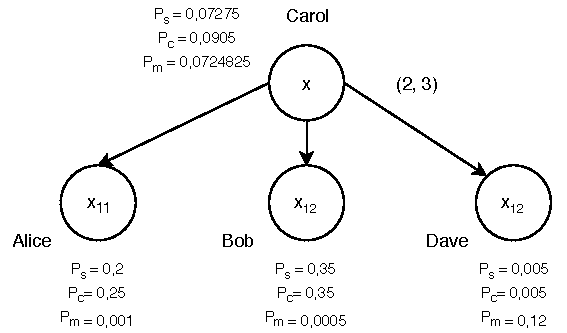
\includegraphics[width=0.6\linewidth]{images/chap_analisi_robustezza/robustezza-1.pdf}
\end{figure}

\paragraph{Albero di distribuzione bilanciato di profondità 2}
Immaginiamo di avere a disposizione quattro agenti. Per tre di questi
vale
$ P_s = 0,1 $ \,
$ P_c = 0,3 $ \,
$ P_m = 0,02 $
mentre per il quarto abbiamo
$ P_s = 0,02 $ \,
$ P_c = 0,02 $ \,
$ P_m = 0,005 $.
Immaginiamo inoltre di utilizzare un albero di distribuzione simmetrico di profondità 2.
Come parametri per l'algoritmo di secret sharing usiamo $ t = 2 $ e $ n = 2 $ in tutti i casi.
La situazione è rappresentata in figura \ref{fig:robustezza-2-1}.

\begin{figure}[H]
	\centering
	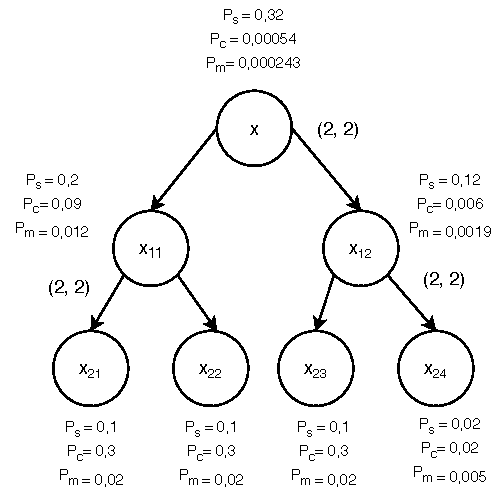
\includegraphics[width=0.6\linewidth]{images/chap_analisi_robustezza/robustezza-2-1.pdf}
	\caption{Albero di distribuzione bilanciato di profondità 2}
	\label{fig:robustezza-2-1}
\end{figure}

Calcoliamo gli attributi di $ x_{11} $. Abbiamo $ t = 2 $ e $ n = 2 $.
La resistenza agli smarimenti è $ \gamma = 0 $,
di conseguenza la $ P_s $ di $ x_{11} $ è data dalla somma delle $ P_s $ dei nodi figli.
$$ P_s = 0,1 + 0,1 = 0,2 $$

Per poter ottenere lo share $ x_{11} $ un attaccante esterno deve riuscire ad ottenere
sia $ x_{21} $ sia $ x_{22} $. Pertanto $ P_c $ è dato dal prodotto dei $ P_c $ dei nodi figli.
$$ P_c = 0,3 \cdot 0,3 = 0,09 $$

Se invece è uno degli agenti a voler ottenere $ x_{11} $  è sufficiente che ottenga
lo share dell'altro agente. Quindi $ P_m $ è data dalla somma delle probabilità
che si abbia sia un agente scorretto sia un agente corrotto.
$$ P_m = (0,02 \cdot 0,3) + (0,02 \cdot 0,3) = 0,0012 $$

Per quanto riguarda gli attributi di $ x_{12} $ abbiamo anche qui $ t = 2 $ e $ n = 2 $.
Il ragionamento è analogo a quello di cui sopra. Ci limitiamo
a riportare i calcoli.
\begin{tightcenter}
	$ P_s = 0,1 + 0,02 = 0,12 $      \\
	$ P_c = 0,3 \cdot 0,02 = 0,006 $ \\
	$ P_m = (0,02 \cdot 0,02) + (0,005 \cdot 0,3) = 0,0019 $
\end{tightcenter}
A questo punto dobbiamo trovare gli attributi di $ x $.
Si ha $ t = 2 $ e $ n = 2 $, anche qui il ragionamento è analogo a prima.
\begin{tightcenter}
	$ P_s = 0,2 + 0,12 = 0,32 $\\
	$ P_c = 0,09 \cdot 0,006 = 0,00054 $\\
	$ P_m = (0,012 \cdot 0,006) + (0,0019 \cdot 0,09) = 0,000243 $
\end{tightcenter}

\paragraph{Albero di distribuzione con ridondanza}
Analogamente al caso precedente immaginiamo di avere a disposizione quattro agenti. Per tre di questi
vale
$ P_s = 0,1 $ \,
$ P_c = 0,3 $ \,
$ P_m = 0,02 $
mentre per il quarto abbiamo
$ P_s = 0,02 $ \,
$ P_c = 0,02 $ \,
$ P_m = 0,005 $.
Immaginiamo inoltre di utilizzare un albero di distribuzione simmetrico di profondità 2.
A differenza del caso precedente però utilizziamo $ t = 1 $ come threshold per gli share di secondo livello.
Facciamo notare che $ t = 1 $ significa che basta un solo share per ricostruire il messaggio originale,
ossia lo share è il messaggio originale. Di fatto possiamo vedere questa situazione come una
distribuzione degli share di primo livello ridondanti.
La situazione è rappresentata in figura \ref{fig:robustezza-2-2}.

\begin{figure}[H]
	\centering
	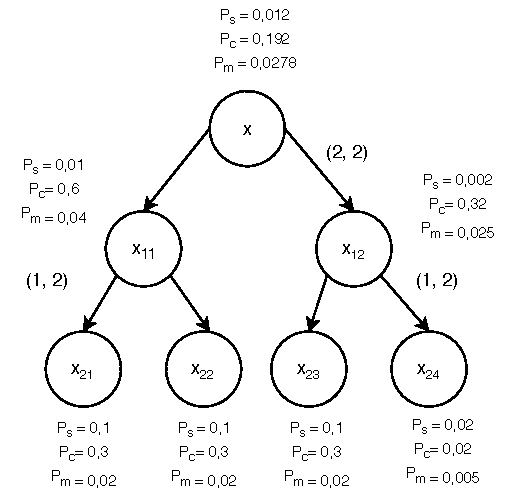
\includegraphics[width=0.6\linewidth]{images/chap_analisi_robustezza/robustezza-2-2.pdf}
	\caption{Albero di distribuzione con ridondanza}
	\label{fig:robustezza-2-2}
\end{figure}

Calcoliamo gli attributi di $ x_{11} $. Abbiamo $ t = 1 $ e $ n = 2 $.
Di fatto $ x_{11} $ è distribuito due volte, quindi
$ x_{11} $ viene smarrito se e solo se entrambi $ x_{21} $ e $ x_{22} $ vengono smarriti.
Di conseguenza per trovare
$ P_s $ dobbiamo moltiplicare i $ P_s $ dei nodi figli.
$$ P_s = 0,1 \cdot 0,1 = 0,01 $$


Per poter ottenere lo share $ x_{11} $ un attaccante esterno deve riuscire ad ottenere
o $ x_{21} $ o $ x_{22} $. Pertando $ P_c $ è dato dalla somma dei $ P_c $ dei nodi figli.
\begin{tightcenter}
	$ P_c = 0,3 + 0,3 = 0,6 $
\end{tightcenter}

Entrambi gli agenti di fatto conoscono $ x_{11} $, quindi per calcolare $ P_m $ si devono
sommare le $ P_m $ dei nodi figli.
\begin{tightcenter}
	$ P_m = 0,02 \cdot 0,02 = 0,04$
\end{tightcenter}

Per quanto riguarda gli attributi di $ x_{12} $ si ha $ t = 1 $ e $ n = 2 $,
i ragionamenti sono analoghi.
\begin{tightcenter}
	$ P_s = 0,1 \cdot 0,02 = 0,002 $\\
	$ P_c = 0,3 + 0,02 = 0,32 $\\
	$ P_m = 0,02 + 0,005 = 0,025 $
\end{tightcenter}

Non ci resta che trovare gli attributi di $ x $.
Abbiamo $ t = 2 $ e $ n = 2 $, il ragionamento è analogo a quello presente nell'esempio precedente.
\begin{tightcenter}
	$ P_s = 0,01 + 0,002 = 0,012 $\\
	$ P_c = 0,6 \cdot 0,32 = 0,192 $\\
	$ P_m = (0,04 \cdot 0,32) + (0,025 \cdot 0,6) = 0,0278 $\\
\end{tightcenter}
TODO confrontare i risultati ottenuti col caso precedente


\paragraph{Albero di distribuzione sbilanciato di profondità 2}
Ancora una volta immaginiamo di avere a disposizione quattro agenti. Per tre di questi
vale
$ P_s = 0,1 $ \,
$ P_c = 0,3 $ \,
$ P_m = 0,02 $
mentre per il quarto abbiamo
$ P_s = 0,02 $ \,
$ P_c = 0,02 $ \,
$ P_m = 0,005 $.
Questa volta però immaginiamo di utilizzare l'albero di distribuzione degli share
sbilanciato di profondità 2
mostrato in figura \ref{fig:robustezza-2-3}.
\begin{figure}[H]
	\centering
	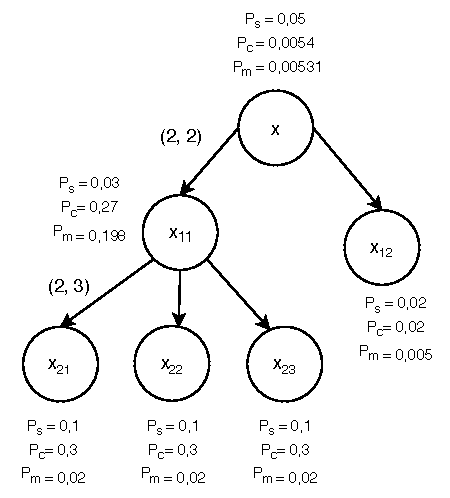
\includegraphics[width=0.6\linewidth]{images/chap_analisi_robustezza/robustezza-2-3.pdf}
	\caption{Albero di distribuzione sbilanciato di profondità 2}
	\label{fig:robustezza-2-3}
\end{figure}
Per prima cosa cerchiamo gli attributi di $ x_{11} $.
Abbiamo $ t = 2 $ e $ n = 3 $. La resistenza agli smarrimenti è $ \gamma = 1 $, perciò $ P_s $
è la somma delle probabilità delle tre combinazioni di avere $ \gamma + 1 = 2 $ smarrimenti.
\begin{tightcenter}
	$ P_s = (0,1 \cdot 0,1) + (0,1 \cdot 0,1) + (0,1 \cdot 0,1) = 0,03 $
\end{tightcenter}

La resistenza ai furti è $ \theta = 2 $. Un attaccante deve recuperare
due share per ottenere $ x_{11} $. Quindi
$ P_s = (0,3 \cdot 0,3) + (0,3 \cdot 0,3) + (0,3 \cdot 0,3) = 0,27 $

Infine $ P_m $ è
$$
	P_m = (0,02 \cdot 0,3) + (0,02 \cdot 0,3) +
	(0,02 \cdot 0,3) + (0,02 \cdot 0,3) +
	(0,02 \cdot 0,3) + (0,02 \cdot 0,3) = 0,198
$$
Non ci resta che trovare gli attributi di $ x $.
Ancora una volta $ t = 2 $ e $ n = 2 $.
\begin{tightcenter}
	$ P_s = 0,03 + 0,02 = 0,05 $      \\
	$ P_c = 0,27 \cdot 0,02 = 0,0054 $\\
	$ P_m = (0,198 \cdot 0,02) + (0,005 \cdot 0,27) = 0,00531 $
\end{tightcenter}



\subsection{Considerazioni}
Questo modello può essere usato come un comodo strumento in grado di fornire
un'indicazione quantitativa sulla robustezza di una data implementazione.
Si tratta però di una approssimazione,
che non tiene conto di alcune dinamiche che si possono venire a creare. Infatti per poter
applicare questa tecnica di analisi si deve assumere che tutti gli agenti siano entità ben distinte
e che non vi siano coalizioni tra agenti. Inoltre è necessario attribuire a priori
$ P_s $, $ P_c $ e $ P_m $ ad ogni agente. Nella pratica questa è una attività non banale.

% In questo capitolo analizzeremo le principali criticità a cui il protocollo
% proposto è esposto. Per chiarezza di esposizione presenteremo
% i diversi scenari divisi per punti, ma è bene
% sapere che alcune di queste situazioni potrebbero verificarsi anche contemporanemente.

% \section{Comportamenti negligenti dei singoli utenti}
% \subsection{Uno o più agenti perdono il segreto}


% \subsection{L'agente si fa rubare il segreto}

% \subsection{Il client si fa rubare/pubblica il segreto prima di $ \tau $}


% \section{Comportamenti malevoli dei singoli utenti}
% \subsection{Comportamento malevole del client}

% \subsection{Comportamento malevolo di un agente}


% \section{Coalizioni tra agenti}


% \section{Un singolo attore controlla più agenti}
% DLT PERMISSIONED
% Affinché il protocollo funzioni al meglio
% è bene che tutti gli $ N $ agenti
% siano entità ben distinte. Purtroppo non in tutti i contesti
% questa caratteristica è facile da verificare.
% Possono quindi venirsi a creare situazioni nelle quali un unico soggetto controlla
% più agenti. Fissato $ k $ il numero di agenti che controlla,
% individuiamo due casi:
% \paragraph{Un singolo soggetto controlla $ k < \gamma $ agenti}
% In questo caso il soggetto non dispone di un numero sufficiente di share per
% ricostruire il segreto. Bisogna considerare però che parte da una posizione di
% vantaggio, perché deve recuperare solo altri $ \gamma - k $ share.
% \paragraph{Un singolo soggetto controlla $ k \geq \gamma $ agenti}
% In questo caso il soggetto dispone di un numero sufficiente di share per
% ricostruire il segreto. Significa che sin dal momento dell'inizializzazione
% del protocollo viene meno il requisito di
% segretezza del messaggio [vedi \ref{parag:segretezza-tre}].


% \section{Un soggetto corrompe gli agenti}
% Un attaccante che vuole ottenere il messaggio prima del tempo $ \tau $ deve riuscire
% ad ottenere almeno $ \gamma $ share.

% Un tecnica che può usare è quella di "corrompere" un numero $ \gamma $ di agenti.
% Per farlo deve offrire ad ogni agente una cifra maggiore di \textit{prize}.
% L'agente ha interesse nel tenere il proprio share segreto perché sa che se lo fa
% al tempo $ \tau $ può ottenere una ricompensa \textit{prize}.
% Se però un soggetto gli
% offre una cifra maggiore o uguale di \textit{prize} a quel punto l'azione
% più conviente diventa cedere il segreto.

% Come è possibile difendersi? Quello che può fare il client è fissare dei
% \textit{prize} adeguatamente alti rispetto al valore del segreto.
% Un'altra tecnica che può aiutare è quella di
% apportare un'ulteriore penalizzazione nel
% caso in cui l'agente ceda il segreto. Queste penalizzazioni possono essere
% legate al particolare dominio applicativo in cui il protocollo viene utilizzato.
% Un esempio è visibile nell'ultimo capitolo. TODO
\chapter{Applicazioni della Timed-Release Encryption}
\label{chap:possibili-usi}

In questo capitolo analizzeremo una serie di possibili
applicazioni della Timed-Release Encryption.

\section{Offerte in aste a buste chiuse}
Spesso per l'assegnazione di bandi pubblici si ricorre all'uso di
offerte a buste chiuse. Il funzionamento è il seguente.
Vengono fissati i requisiti minimi che devono essere soddisfatti
dalle offerte, i criteri per l'attribuzione del punteggio alle offerte e una scadenza.
A questo punto ogni partecipante presenta all'ente pubblico
la propria offerta in forma cartacea
all'interno di una busta sigillata, rimanendo
completamente all'oscuro sulla presenza di eventuali altri partecipanti e sul
contenuto delle offerte presentate. Una volta raggiunta la scadenza
le buste vengono aperte, validate, vengono calcolati i punteggi
e viene decretato il vincitore.
I funzionari pubblici coinvolti hanno un ruolo chiave nel processo.
Sono loro a garantire la segretezza e l'integrità
delle offerte fino alla scadenza del bando.
Inoltre devono garantire il rispetto della scadenza per la presentazione delle offerte.
In questo processo talvolta si verificano casi di corruzione.

Una possibile alternativa è l'uso della Timed-Release Encryption. Ogni partecipante
cifra la propria offerta con la TRE, fissando come deadline la scadenza del bando.
Raggiunta la scadenza le offerte vengono automaticamente rese pubbliche. A differenza
del processo di cui sopra l'integrità
e la segretezza delle offerte verrebbero garantite dalla crittografia e non dall'uomo.

\section{Insider stock trades}
Un insider, ossia una persona che può avere accesso in anticipo a informazioni
riservate sull’attività economica di una società quotata in borsa,
potrebbe essere legalmente obbligato a
prendere impegni in anticipo sull'acquisto di quote della società
sia per mitigare potenziali
abusi di informazioni interne, sia per proteggere l'insider da false
accuse di utilizzo sleale delle informazioni.
In certe circostanze
si può volere che questi impegni rimangano segreti sino a poco prima
della loro esecuzione. Chiaramente un impegno che non garantisce la non ripudiabilità
non è sufficiente in quanto un insider può creare in anticipo un impegno nascosto
e poi rifiutarsi di renderlo pubblico nel caso in cui l'evento non sia per lui conveniente.

Se un insider cifra in anticipo la sua transazione con la Timed-Release Encryption
può sempre essere legalmente obbligato a eseguire la transazione e allo stesso tempo
i dettagli della transazione rimangono segreti fino al tempo desiderato.
In \cite{rabin2006time} Rabin e Thorpe propongono un protocollo nel quale gli insider
cifrano le loro transazioni in anticipo usando la Timed-Release Encryption.
Queste direttive possono essere per l'acquisto, per la vendita o non fare nulla. In questo
modo l'insider non rivela informazioni al mercato.

\section{Raccolta dati in trial clinici}
Al fine di preservare l'integrità dei trial clinici, le informazioni raccolte durante il trial
posso essere cifrate con la Timed-Release Encryption.
Poiché molti di questi studi sono finanziati da società che sono in grado di guadagnare
o perdere ingenti somme di denaro a seconda del loro esito,
potenzialmente vi possono essere pressioni per ottenere un risultato positivo.
L'uso della Timed-Release Encryption può mitigare bias senza rendere note informazioni
confidenziali riguardo lo studio prima che sia completato. La Timed-Release Encryption
previene le frodi da parte di scienziati non etici, e protegge gli scienziati onesti
da false accuse di frode o pressioni da parte dei loro finanziatori per ottenere un certo risultato.

In un contesto, i dati raccolti dagli scienziati verrebbero cifrati
immediatamente mentre vengono raccolti dai dispositivi medici. In questo modo gli scienziati
non sarebbero in grado di conoscere i dati prima della conclusione di una certa fase dello studio;
ciò previene che i trend che si verificano nelle prime fasi dello studio influenzino
le successive operazioni di raccolta dati.
In un altro contesto, i dati clinici verrebbero forniti immediatamente agli scienziati
e successivamente ad una commissione di auditing tramite Timed-Release Encryption.
In questo modo gli scienziati non comunicano immediatamente alla commissione i dati raccolti
e allo stesso tempo al termine della sperimentazione
la commissione di auditing ha la garanzia che i dati non siano stati alterati.

\section{Voto elettronico}
In alcune forme di votazioni si desidera che non vi siano pubblicazioni di risultati intermedi,
perché potrebbero influenzare gli altri elettori. Se i voti vengono cifrati con
la Timed-Release Encryption durante la votazione, i risultati possono rimanere interamente segreti
fino alla chiusura delle urne.

% In one setting, scientists’ data collection process uses our Service to encrypt
% data directly as they are being collected, for example, by diagnostic devices
% or computer user interfaces. The scientists would not be able to see the data
% collected until the conclusion of a phase of the study; this prevents observations
% of trends in early data collection from affecting future data collection practices.
% In another setting, clinical data would be provided to the scientists in raw
% form immediately and to an auditing board encrypted via time-lapse cryptography.
% The scientists would preserve the confidentiality of their data during the
% study to prevent leaking of information by the auditing board, but would know
% that any tampering with results would be discovered after the expiration of the
% time-lapse.

% \cite{Rivest96time-lockpuzzles}
% What are the applications of timed-release crypto"? Here are a few possibilities (some
% due to May):
% A bidder in an auction wants to seal his bid so that it can only be opened after the
% bidding period is closed.
% A homeowner wants to give his mortgage holder a series of encrypted mortgage payments.
% These might be encrypted digital cash with different decryption dates, so that
% one payment becomes decryptable (and thus usable by the bank) at the beginning of
% each successive month.
% An individual wants to encrypt his diaries so that they are only decryptable after fty
% years.


% % altro paper
% Bids in sealed-bid auctions. Our original motivation for this work came
% from joint work with David Parkes and Stuart Shieber on cryptographic auctions
% 	[17]. In our auction protocol, we realized the need for bidders to issue

% \section{Gara d'appalto a buste chiuse}
% \label{sec:gara-buste-chiuse}

\appendix
% % INCLUSIONE APPENDICI - - PERSONALIZZARE - TENERE COERENTE CON LISTA IN ALTO

%%%%%%%%%%%%%%%%%%%%%%%%%%%%%%%%%%%%%%%%%%%%%%%%%%%%%%%%%%%%%%%

% BIBLIOGRAFIA
\addcontentsline{toc}{chapter}{\refname}
\nocite{*}
\printbibliography

\end{document}